\documentclass[pdf]{beamer}
\mode<presentation>{
	\usetheme{Copenhagen}
	\usecolortheme{seahorse}
}

\setbeamertemplate{footline}[page number]
\renewcommand{\footnotesize}{\tiny}

%% Language and font encodings
\usepackage[frenchb]{babel}

\usepackage[utf8]{inputenc}
\usepackage[T1]{fontenc}

\usepackage{verbatim}
\usepackage{enumitem}
\usepackage{hyperref}

% bibliography package            
\usepackage[backend = biber, style = numeric]{biblatex}   
\addbibresource{references.bib}            

% pour les images
\usepackage{graphicx}
\usepackage{caption} 
\usepackage{float} 
\usepackage{wrapfig}

\usepackage[colorinlistoftodos]{todonotes}
\usepackage{multimedia}

\title[]{Notation symbolique de flux de contrôle musicaux et multimédia}
\institute[]{Faculté des sciences - Université de Montpellier}
\author[]{Vincent Iampietro\\[2ex] {\small \textit{Encadrants:} \\ Jean Bresson \\ Rama Gottfried}}

\AtBeginSection[]
{
	\begin{frame}[plain]{Sommaire}
	\tableofcontents[currentsection]
	\end{frame}
}

\beamertemplatenavigationsymbolsempty

\begin{document}

\begin{frame}[plain]
	\titlepage
\end{frame}

\begin{frame}[plain]{Sommaire}
	\tableofcontents
\end{frame}

%%%%%%%%%%%%%%%%%%%%%%%%%%%%%%%%%%%%%%%%%%%%%%%%%
%%  DE LA NOTATION DE LA MUSIQUE CONTEMPORAINE %%
%%%%%%%%%%%%%%%%%%%%%%%%%%%%%%%%%%%%%%%%%%%%%%%%%
\section[De la notation]{De la notation de la musique contemporaine}

\subsection[Notation traditionnelle]{La notation traditionnelle occidentale}
\begin{frame}{Exemple de pièce de l'époque romantique}

\begin{figure}
	\centering
	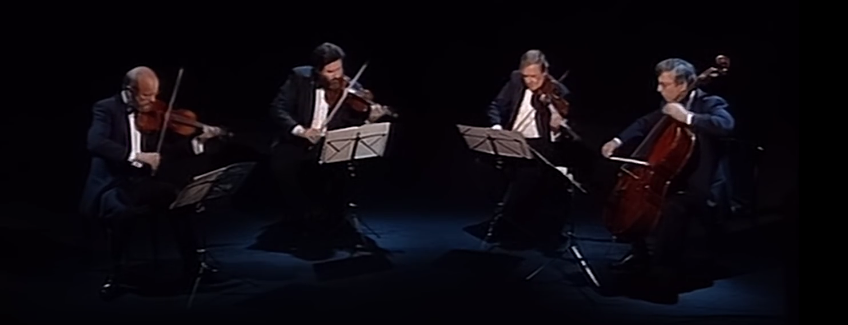
\includegraphics[keepaspectratio=true, width=\textwidth]{./medias/quatuorACordes.png}
	\caption{Le Alban Berg Quartet interprète le Quatuor à cordes No.14 (\textit{La Jeune Fille et la Mort}) (1824), premier mouvement \textit{allegro} de F. P. Schubert \movie[]{
\includegraphics[scale=0.05]{./medias/playButton.png}}{./medias/ChopinMazurkaOp17No4.aiff}}
\end{figure}

\end{frame}

\begin{frame}
	\begin{figure}
		\centering
		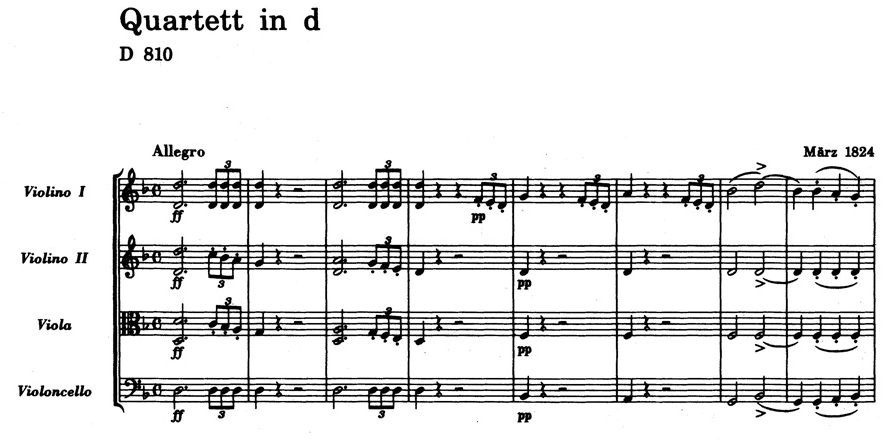
\includegraphics[keepaspectratio=true, width=\textwidth]{./medias/deathAndTheMaiden_extract1.jpg}
		\caption{Extrait de \textit{La jeune fille et la mort}, Franz P. Schubert}
	\end{figure}
\end{frame}

\begin{frame}{Noter la musique}
\begin{figure}
	\centering
	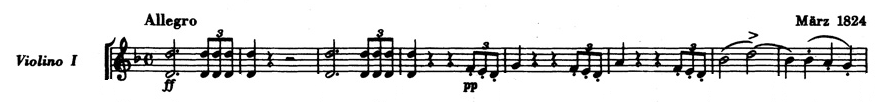
\includegraphics[keepaspectratio=true, width=\textwidth]{./medias/deathAndTheMaiden_extract2.jpg}
\end{figure}
\begin{block}{Le rôle de la partition} 
\begin{itemize}[label={$\square$}]
	\item Un espace de travail pour le compositeur.
	\item Médium de partage, de communication.
\end{itemize}
\end{block}
\begin{block}{Un système unifié (\textit{Common Western Music Notation})}
\begin{itemize}[label={$\square$}]
	\item Système d'écriture basé sur le symbole.
	\item La portée comme structure centrale.
	\item Description de la hauteur, la durée des sons.
\end{itemize}
\end{block}

\end{frame}

\subsection{La musique contemporaine}
\begin{frame}{Qu'est-ce que la musique contemporaine?}

\begin{block}{Définition}
Ensemble des mouvements de musique savante apparus après la seconde guerre mondiale. La musique savante [...] désigne des traditions musicales impliquant des considérations structurelles et théoriques avancées.
\end{block}

\begin{block}{De nouvelles pratiques}
\begin{itemize}[label={$\square$}]
	\item Utilisation de l'électronique/informatique.
	\item Modification du rapport à l'instrument.
	\item Modification du rapport au temps.
\end{itemize}
\end{block}		

\end{frame}

\begin{frame}{Exemple de pièce contemporaine}

\begin{figure}
	\centering
	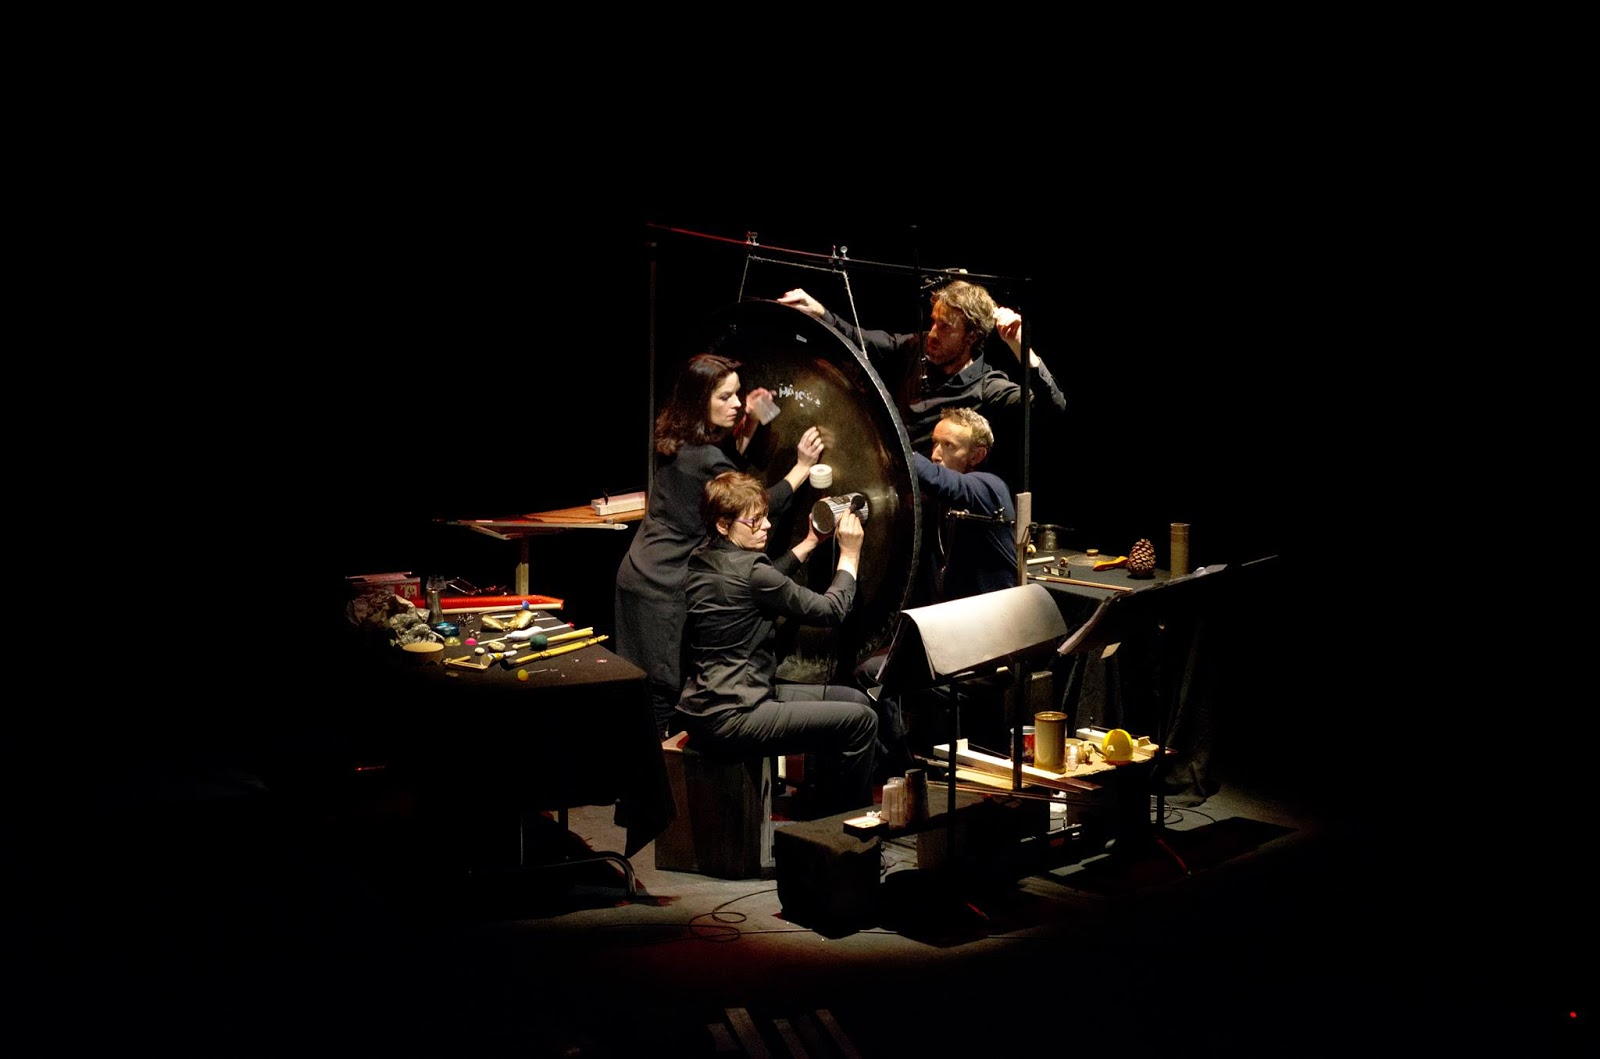
\includegraphics[keepaspectratio=true, width=0.8\textwidth]{./medias/mikrophonie-stockhausen.jpg}
	\caption{En 2016, l'ensemble Sillages interprète \textit{Mikrophonie I} (1964), de K. Stockhausen. \movie[]{
\includegraphics[scale=0.05]{./medias/playButton.png}}{./medias/ChopinMazurkaOp17No4.aiff}}	
\end{figure}

\end{frame}

\begin{frame}
	\begin{figure}
		\centering
		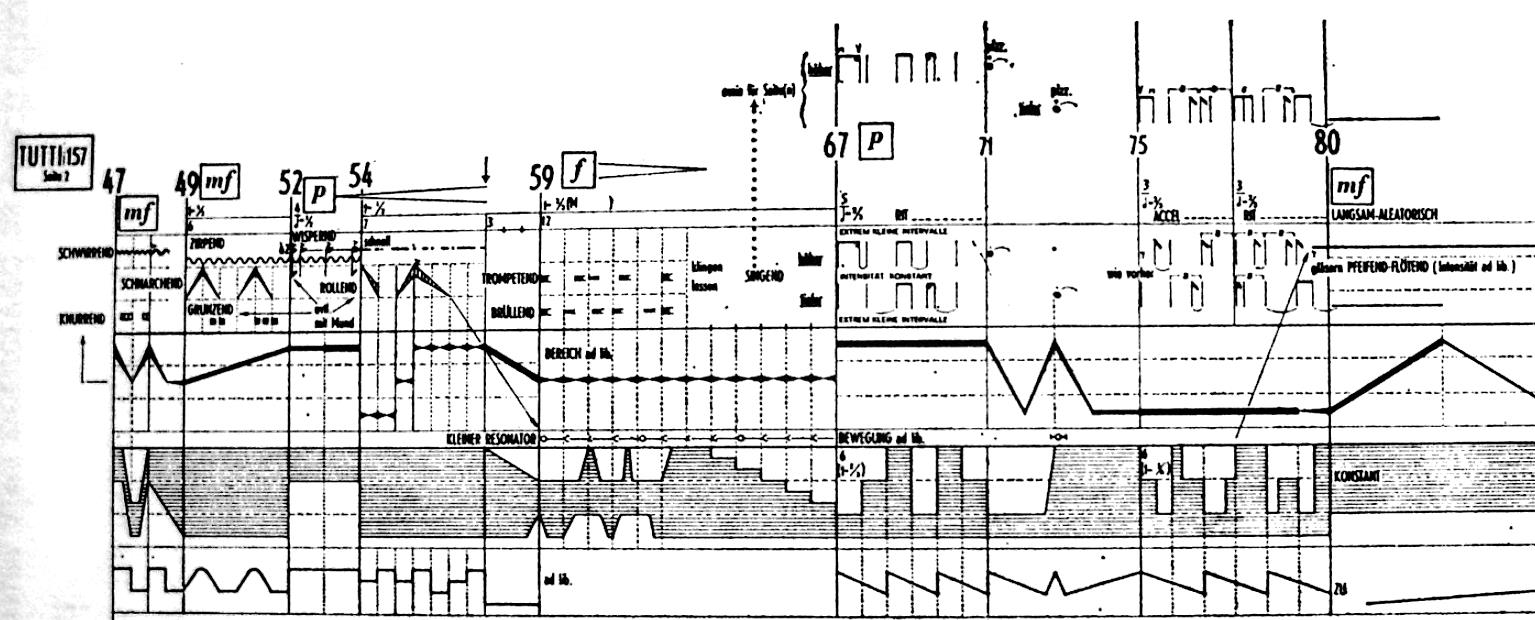
\includegraphics[keepaspectratio=true, width=\textwidth]{./medias/tutti157.jpg}
		\caption{Extrait de la partition de \textit{Mikrophonie I} (1964), mouvement \textit{Tutti 157}, de K. Stockhausen.}	
	\end{figure}
\end{frame}

\begin{frame}{Quel statut pour la partition?}
	\only<1>{
		\begin{figure}
			\centering
			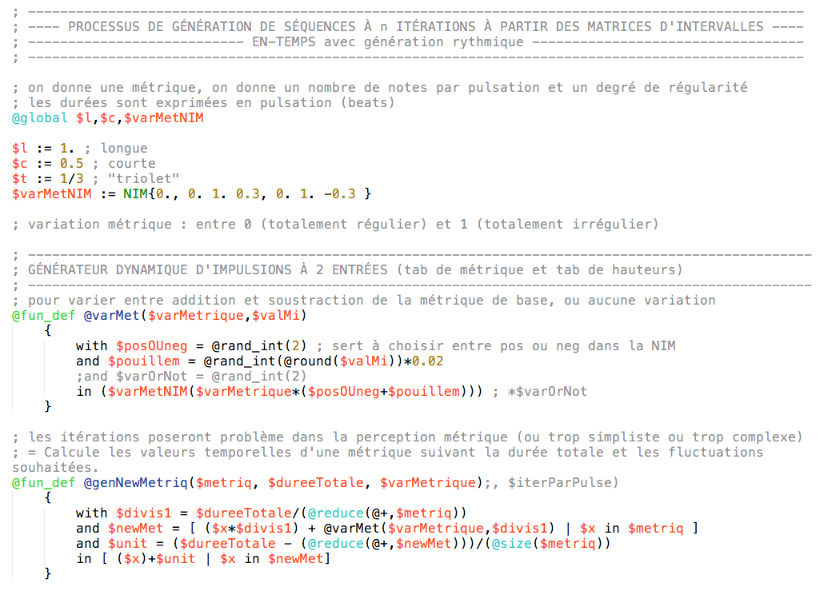
\includegraphics[keepaspectratio=true, width=0.75\textwidth]{./medias/sortirDuNoir.png}
			\caption{Extrait d'un programme, en langage \textit{Antescofo}, décrivant la partie électronique de la pièce \textit{Sortir du noir} (2016), de Julia Blondeau.}	
		\end{figure}
	}
	\only<2>{
		\begin{figure}
			\centering
			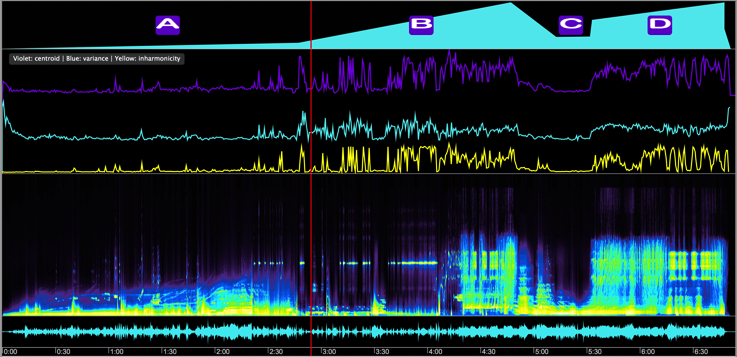
\includegraphics[keepaspectratio=true, width=0.8\textwidth]{./medias/diamorphoses.jpg}
			\caption{Extrait de la pièce \textit{Diamorphoses} (1957), de I. Xenakis, analysée dans le logiciel \textit{EAnalysis}\footfullcite{couprie2018}}	
		\end{figure}
	}
\end{frame}

\begin{frame}{Outils de notation pour la musique contemporaine}
	\begin{figure}
			\centering
			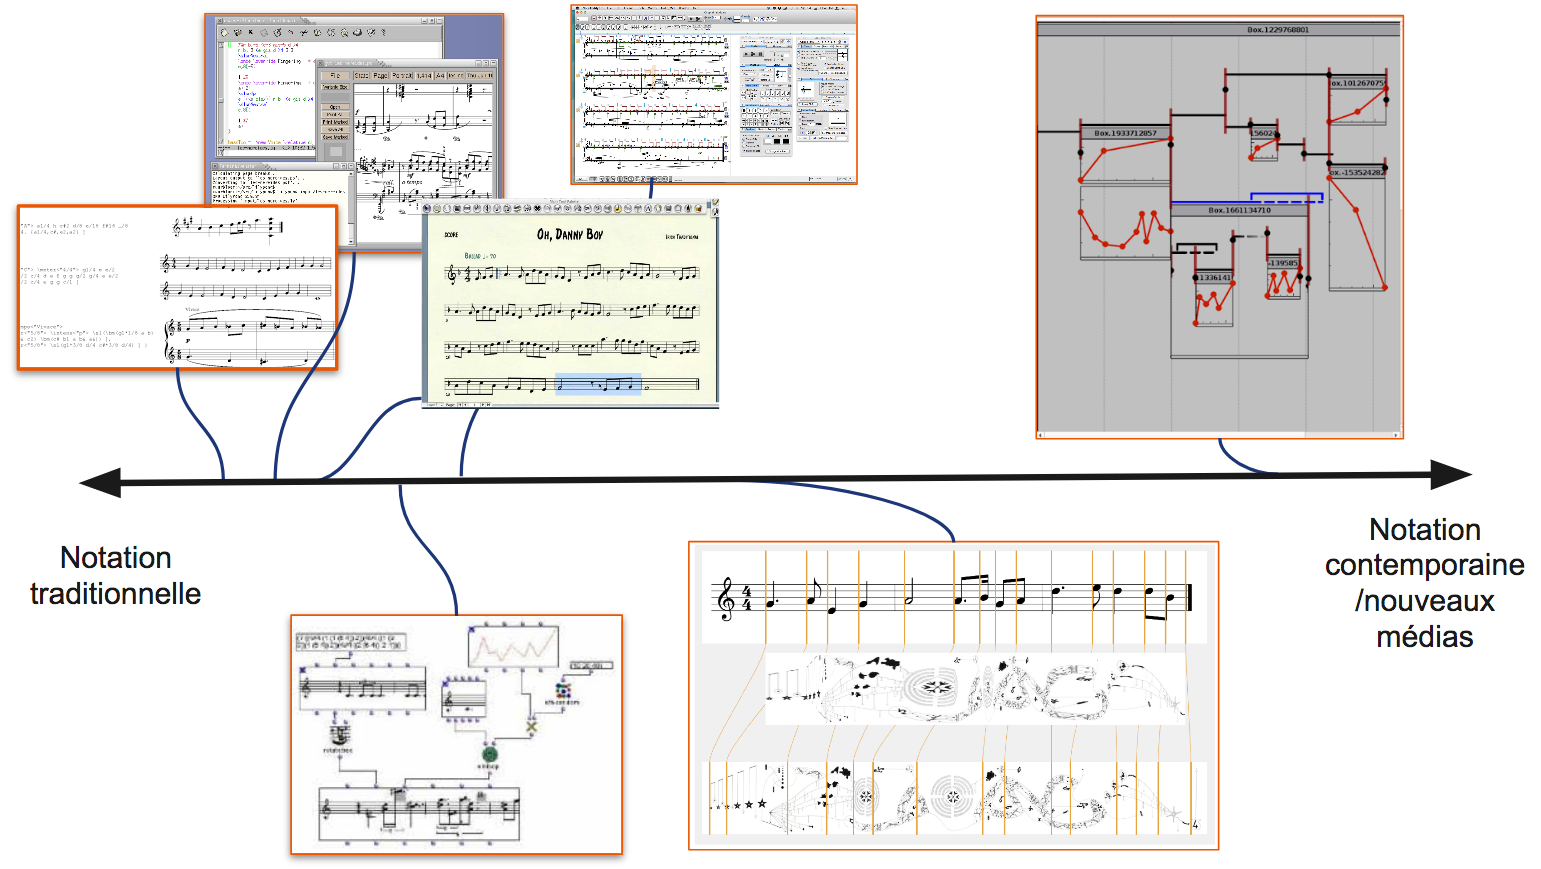
\includegraphics[keepaspectratio=true, width=\textwidth]{./medias/classificationLogiciels.png}
			\caption{Classification des logiciels de notation musicale}	
	\end{figure}
\end{frame}

\begin{frame}{Problématiques}
	\begin{block}{Pour résumer} 
		\begin{itemize}[label={$\square$}]
			\item Nouvelles pratiques musicales.
				  \begin{itemize}
				  	\item \small électronique/informatique, gestes, temps multiples.
				  \end{itemize}				   
			\item Nouvelles formes de notation.
				  \begin{itemize}
				  	\item \small graphique, textuelle, morphologique.
				  \end{itemize}
			\item Pas d'unification des systèmes de notation.
			\item Lacunes des outils logiciels.
				  \begin{itemize}
				  	\item \small restent sur des paradigmes anciens, ou trop spécifiques.
				  \end{itemize}
		\end{itemize}
	\end{block}
	\begin{block}{Axes de recherche} 
		\begin{itemize}[label=$\square$]
			\item Créer un outil qui répond aux besoins des compositeurs.
			\item Créer un outil qui aide à reconsidérer la place de la partition dans la création musicale contemporaine.
		\end{itemize}
	\end{block}
\end{frame}

%%%%%%%%%%%%%%%%%%%%%%%%%%
%%  LE PROJET SYMBOLIST %%
%%%%%%%%%%%%%%%%%%%%%%%%%%
\section[Symbolist]{Le projet symbolist}

\subsection{Présentation du projet symbolist}
\begin{frame}{Présentation du logiciel symbolist}
	\only<1>{
		\begin{figure}
			\centering
			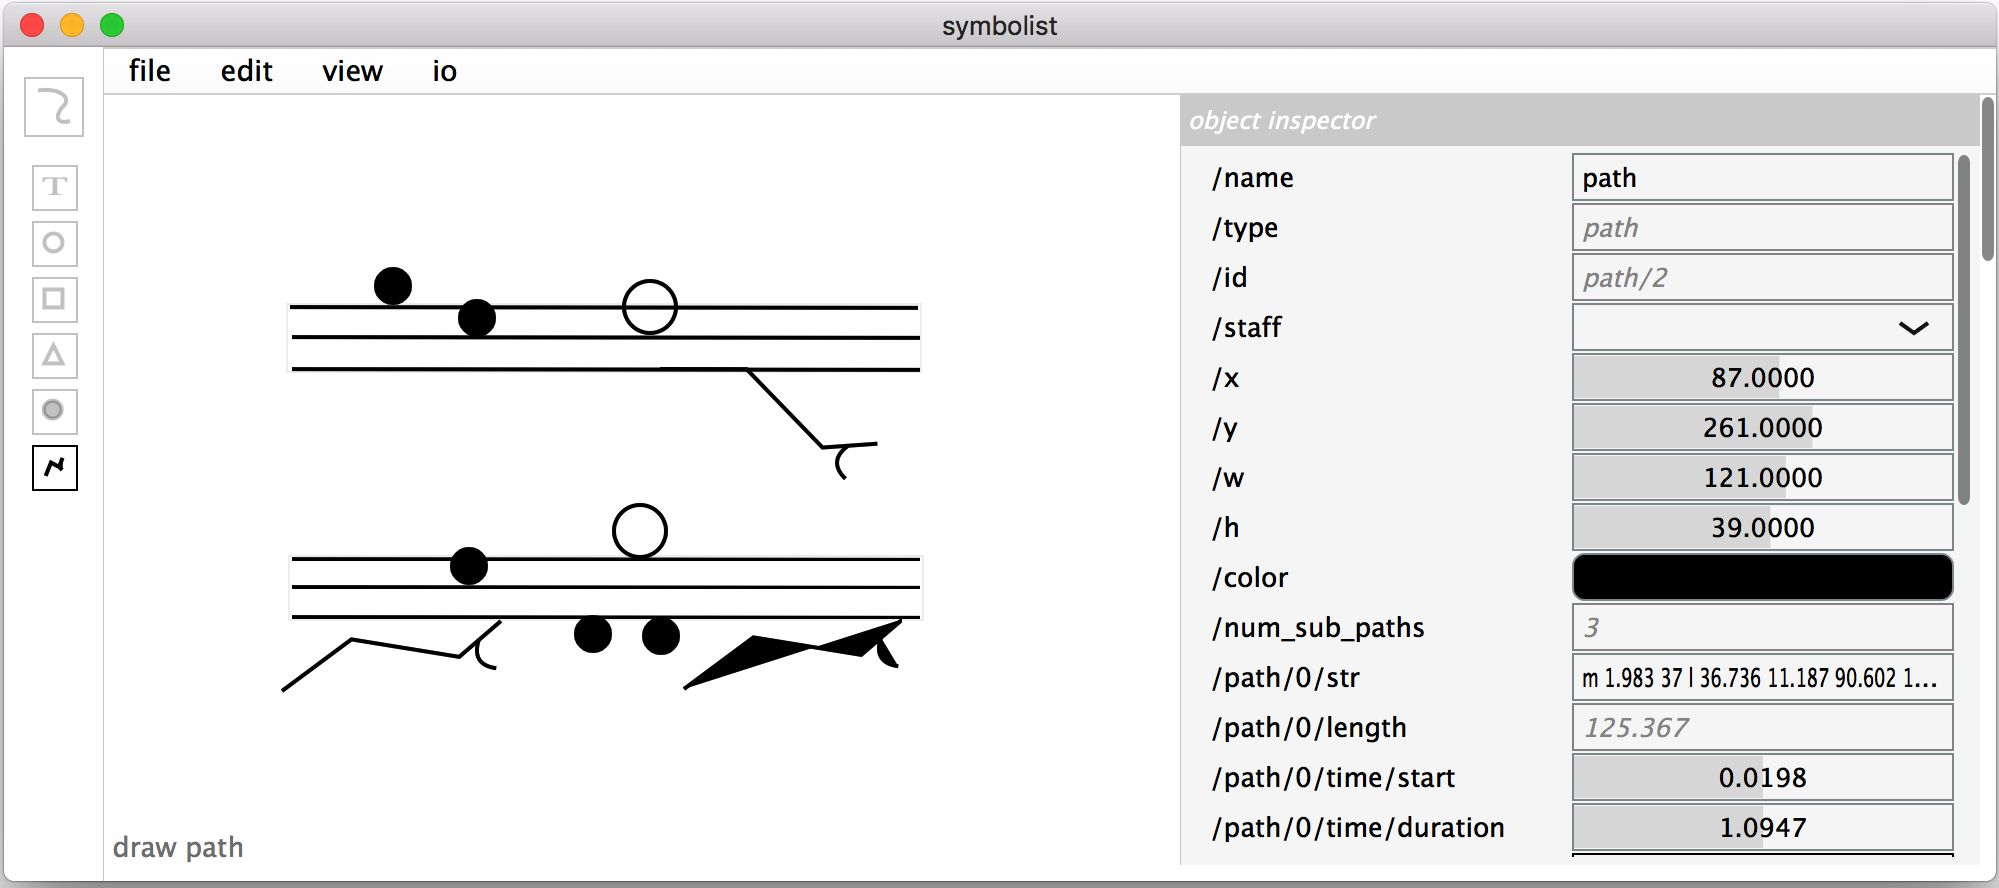
\includegraphics[keepaspectratio=true, width=\textwidth]{./medias/screen-staves.png}
			\caption{Interface du logiciel \textit{symbolist}}	
		\end{figure}
	}	
	
	\only<2>{		
		\begin{itemize}[label={$\square$}]
			\item Le symbole au centre de la démarche.
			\item Canevas d'expression libre.
			\item Interopérabilité (le format \textit{Open Sound Control}\footfullcite{wright2005}, OSC).
		\end{itemize}
		\begin{figure}
			\centering
			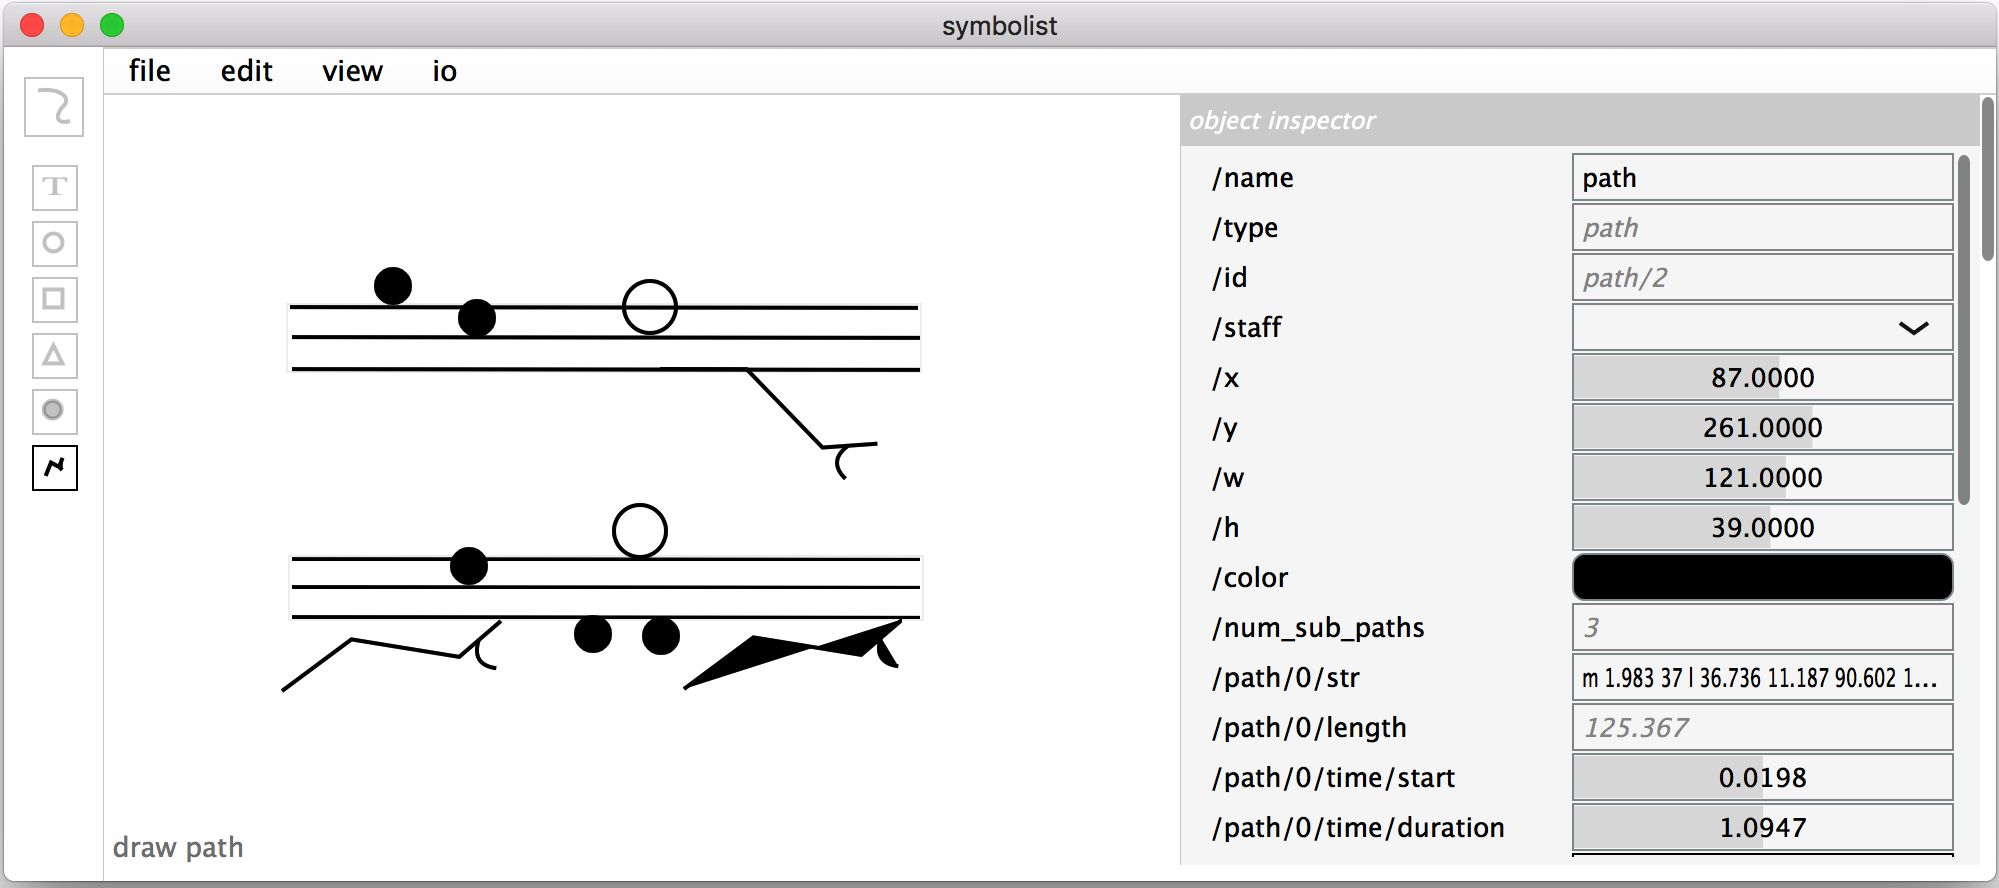
\includegraphics[keepaspectratio=true, width=0.8\textwidth]{./medias/screen-staves.png}
		\end{figure}	
	}
\end{frame}

\begin{frame}{Contributions}
	\begin{itemize}[label=$\square$]
		\only<1->{\item Restructuration logicielle.}
		\only<2->{\item Intégration de la notation traditionnelle.}
		\only<3->{\item Utilisation des expressions \textit{odot}}
		\begin{itemize}[label={$\rightarrow$}]
			\only<1>{\item Architecture MVC, design patterns (composite, command…). }  
			\only<2>{\item \textit{Standard Music Font Layout} (SMuFL), et la police \textit{Bravura}.}
			\only<3>{\item Les adresses OSC comme variables d'expressions.}
		\end{itemize}
	\end{itemize}
	\only<1>{
		\begin{figure}
			\centering
			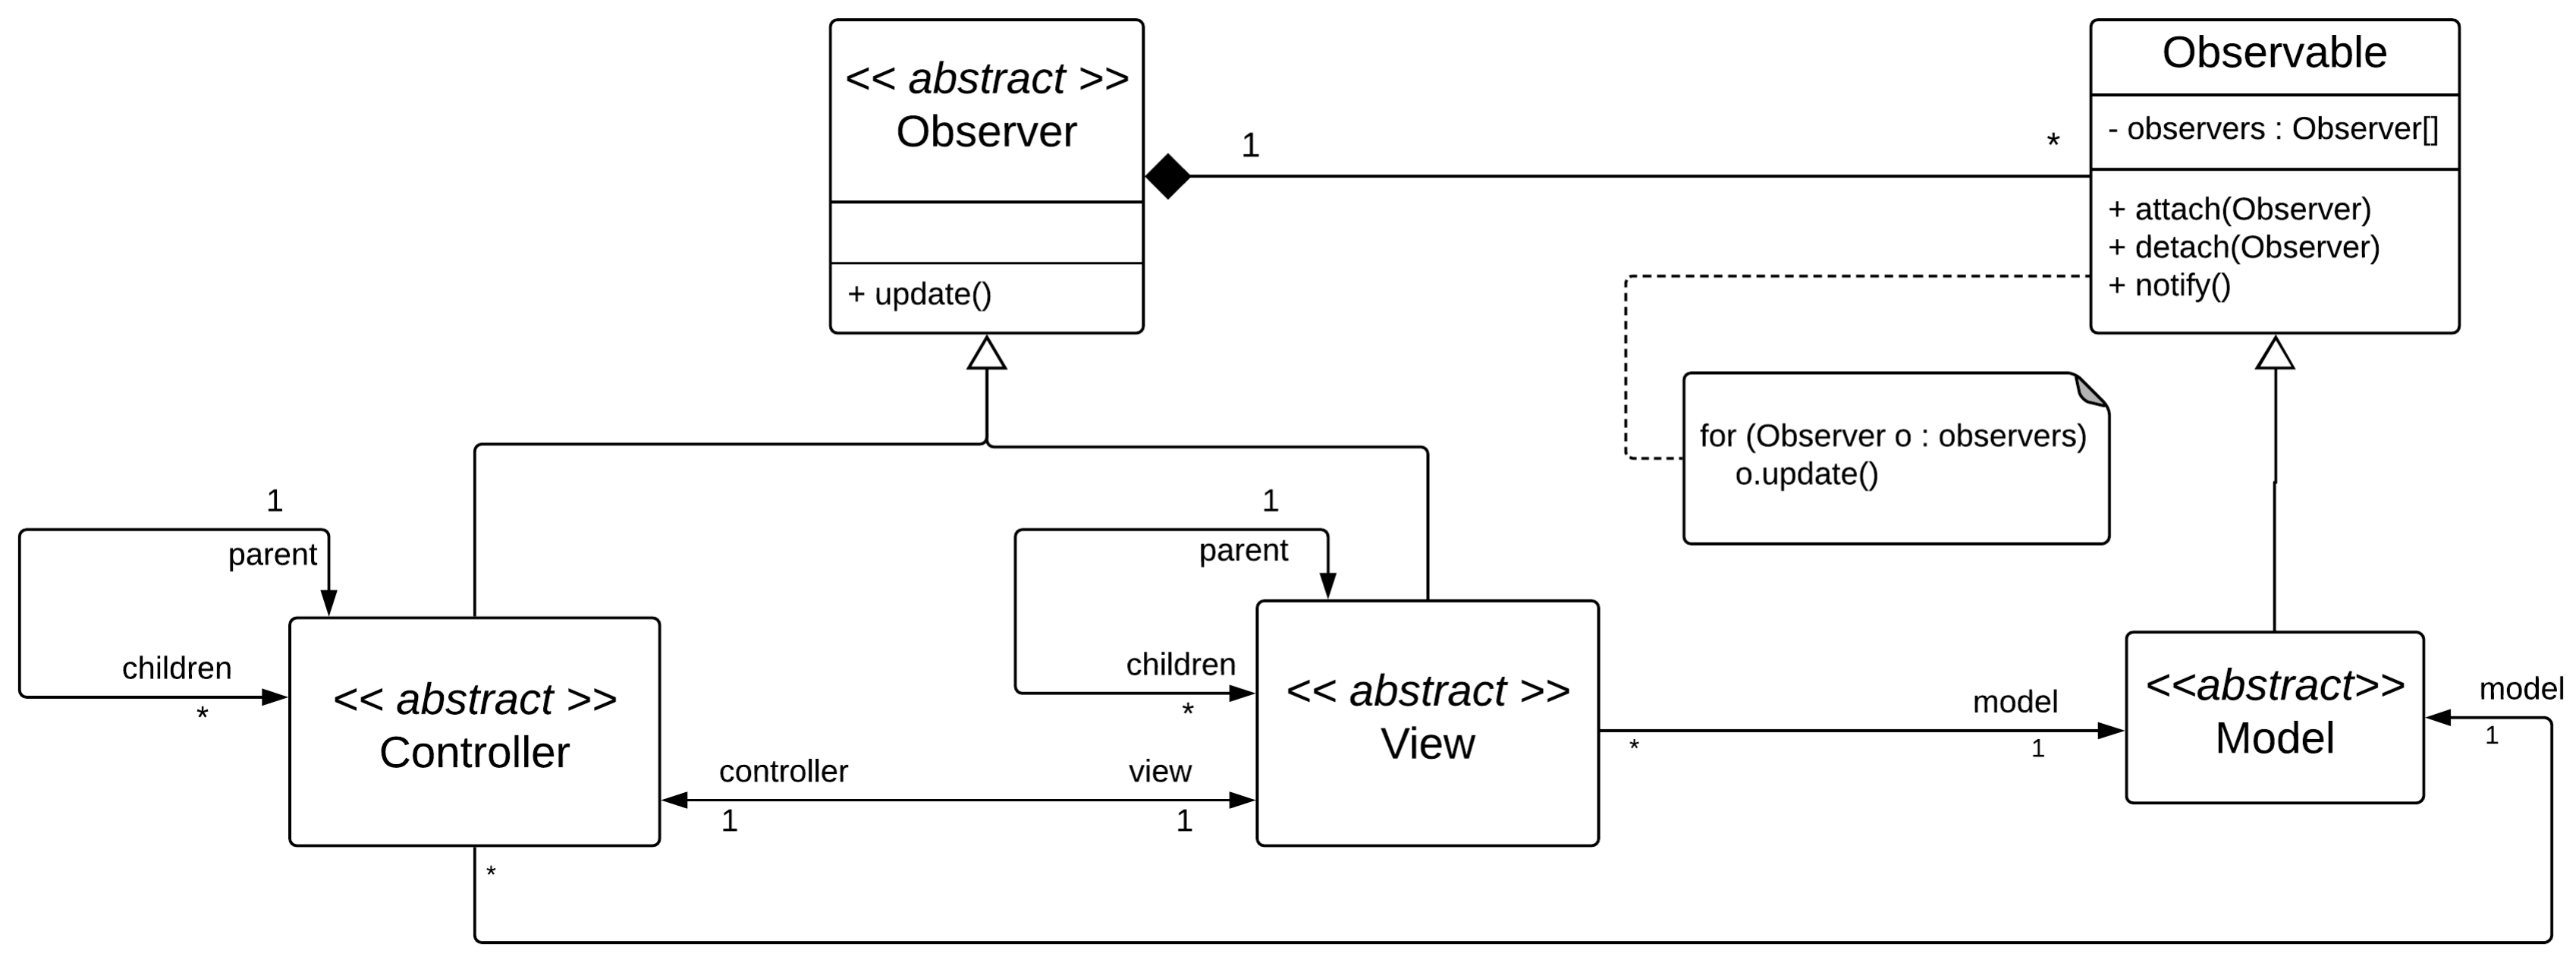
\includegraphics[keepaspectratio=true, width=\textwidth]{./medias/mvcApi.png}
		\end{figure}	
	}
	\only<2>{
		\begin{figure}
			\centering
			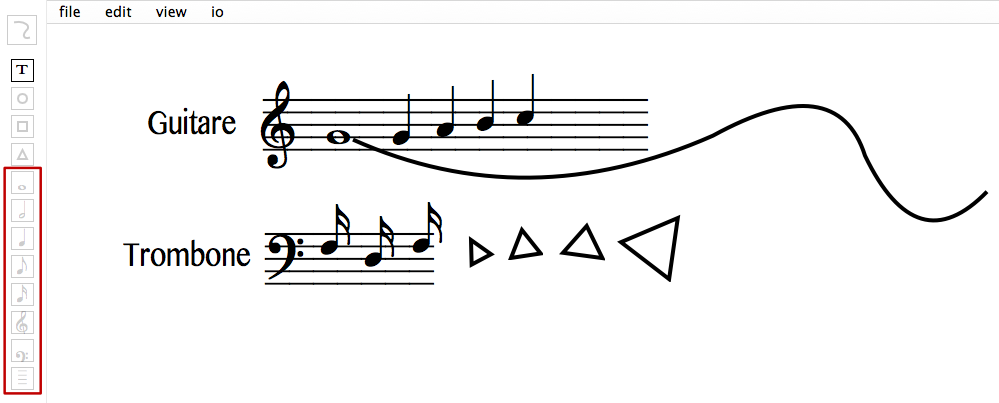
\includegraphics[keepaspectratio=true, width=\textwidth]{./medias/bravuraCreation.png}
		\end{figure}	
	}
	\only<3>{
		\begin{figure}
			\centering
			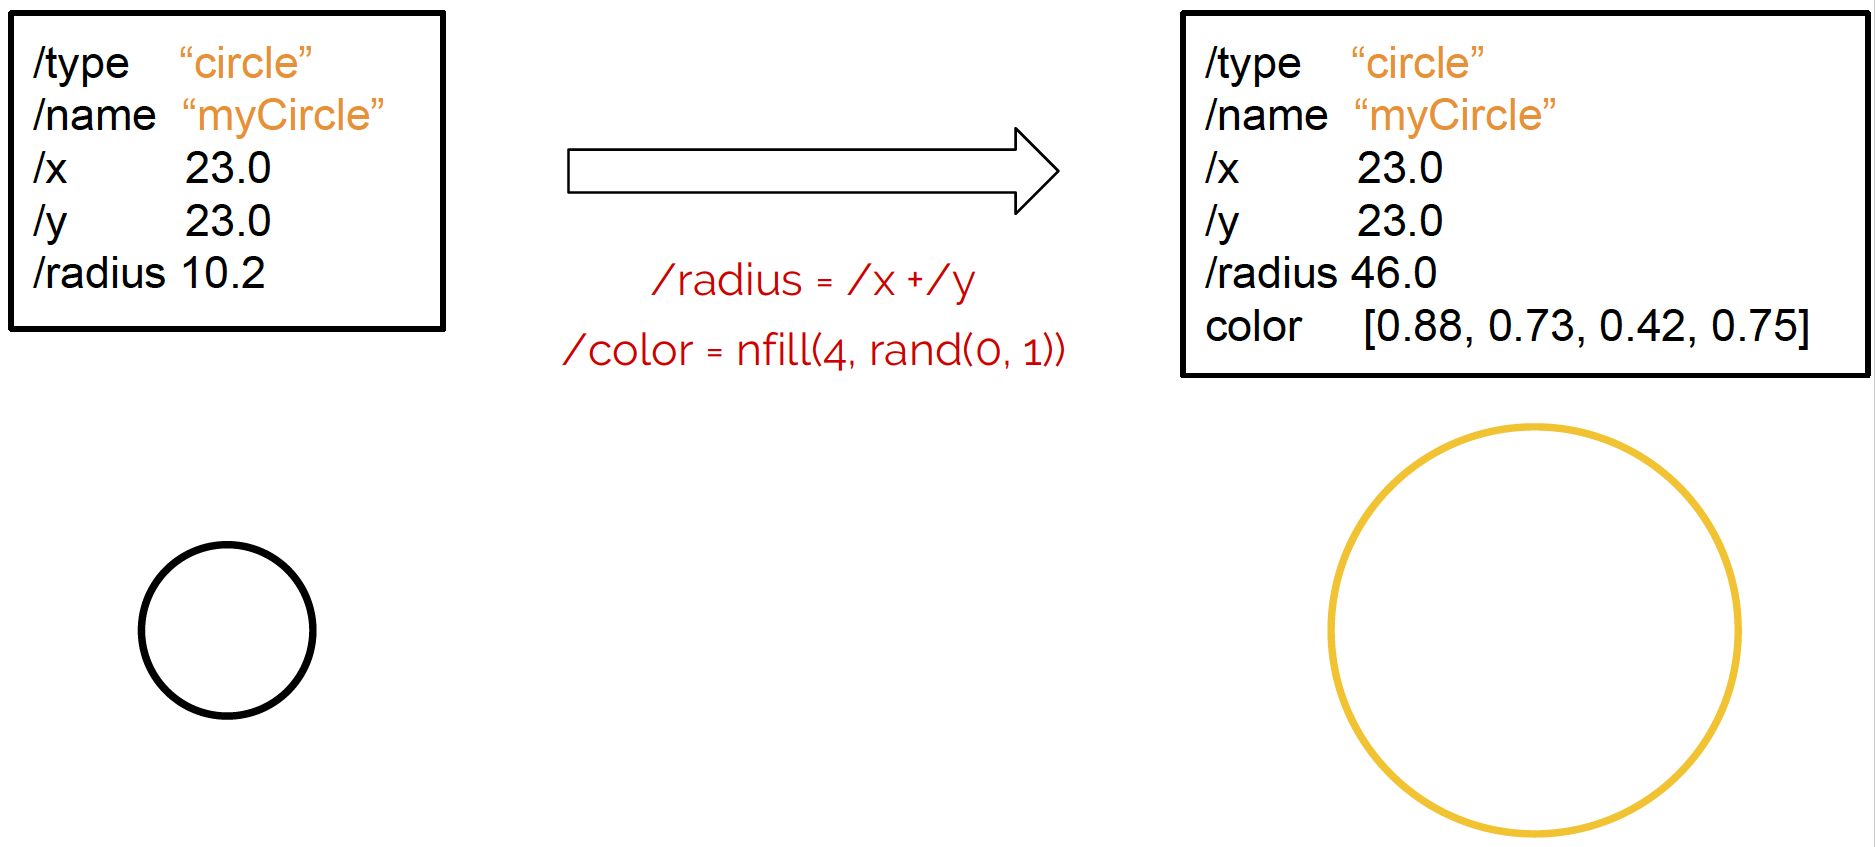
\includegraphics[keepaspectratio=true, width=\textwidth]{./medias/odotExprWithSymbol.png}
		\end{figure}	
	}
\end{frame}

\subsection{Vers une notation exécutable}
\begin{frame}{Le concept de notation exécutable}
Deux sens…
\begin{block}{Exécution sonore}
La partition peut-être perçue comme un pilote des paramètres de la production du son.
\end{block}
\begin{block}{Exécution fonctionnelle}
Les symboles et structures de la partition contiennent de l'intelligence programmationnelle pour modifier cette même partition.
\end{block}
\end{frame}

\begin{frame}{Exécution sonore}
	\begin{itemize}[label=$\square$]
		\item Faire la liaison entre les paramètres graphiques de la partition et les paramètres de contrôle d'instruments.
		\item Un instrument peut être tout type d'entité sachant interpréter les messages OSC.
		\item Liaison entre \texttt{/y} et \texttt{/pitch}: \texttt{/pitch}$ = f($\texttt{/y}$(t))$
		% \item Ordonnancement temporel par le staff.
	\end{itemize}

	\begin{figure}
		\centering
		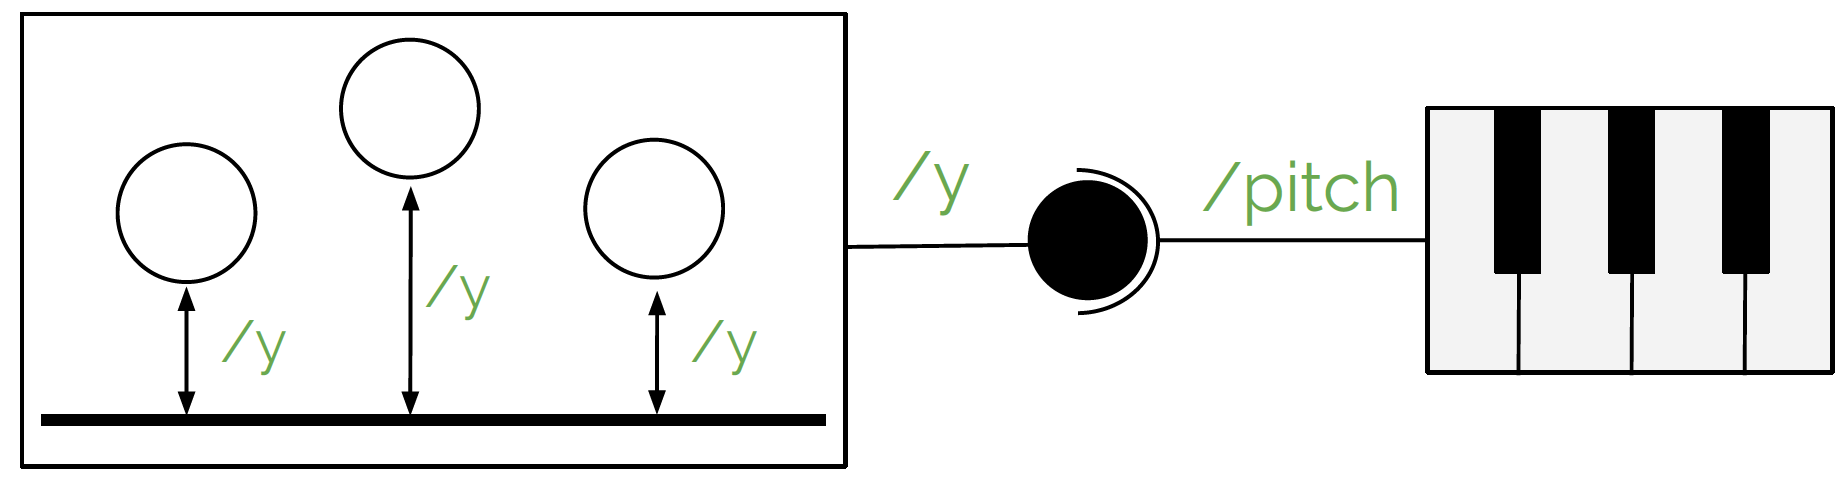
\includegraphics[keepaspectratio=true, width=\textwidth]{./medias/linkingParameters.png}
	\end{figure}	
\end{frame}

\begin{frame}{Exécution fonctionnelle}
	\begin{itemize}[label=$\square$]
		\item Le symbole comme conteneur d'expressions \textit{odot}.
		\item Application d'expressions à un ensemble de symboles : le concept de clef.
	\end{itemize}
	\begin{figure}
		\centering
		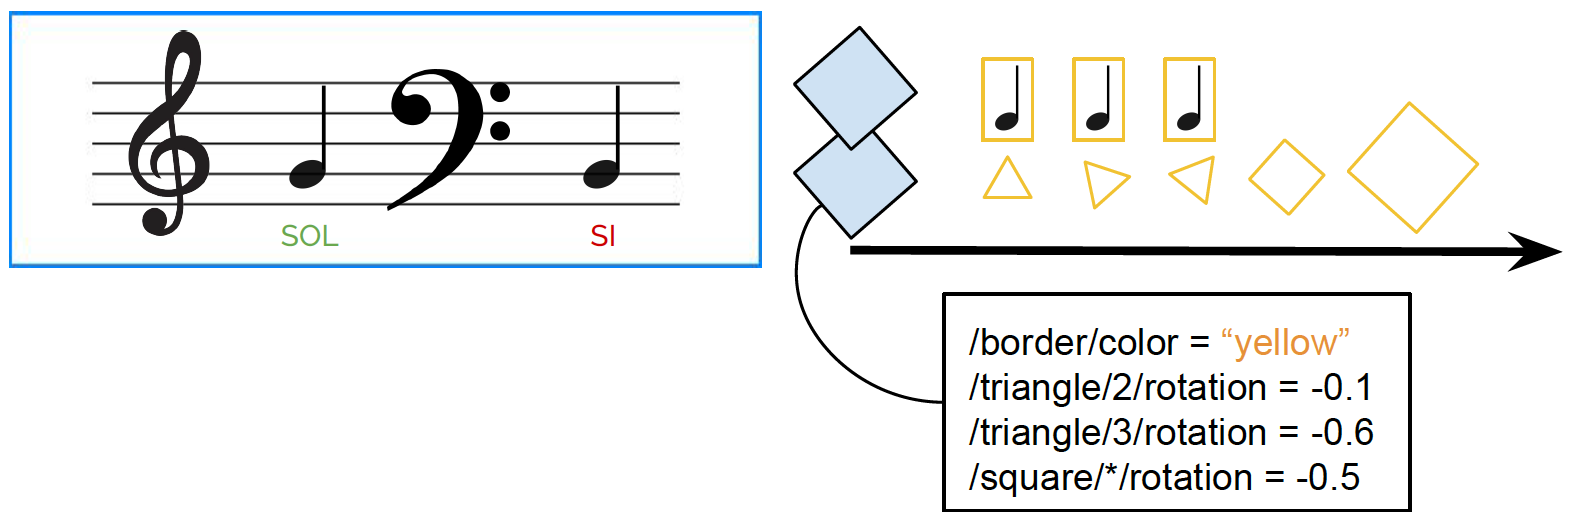
\includegraphics[keepaspectratio=true, width=\textwidth]{./medias/conceptDeClef.png}
	\end{figure}
\end{frame}

\begin{frame}{Démonstration}
\begin{exampleblock}{Vers une notation exécutable avec symbolist.}
	\begin{itemize}[label={$\square$}]
		\item Exemple d'exécution sonore. 
		\item Exemple d'exécution fonctionnelle.
	\end{itemize}
\end{exampleblock}

\end{frame}

%%%%%%%%%%%%%%%%%%%%%%%%%%
%%       CONCLUSION     %%
%%%%%%%%%%%%%%%%%%%%%%%%%%
\section{Conclusion}
\begin{frame}{Apport à la recherche en informatique musicale}
 \begin{itemize}[label=$\square$]
 	\item \textit{symbolist} propose un modèle de notation ouvert.
 	\item Centré sur le symbole, pour l'humain, et sur le format OSC, pour la machine.
 	\item Un pas vers la notation exécutable avec les expressions \textit{odot}.
 \end{itemize}
\end{frame}

\begin{frame}{Perspectives pour symbolist}
 \begin{itemize}[label=$\square$]
 	\item Vers une composition des interfaces de la partition et des systèmes de production sonore.
 	\item Intégration complète de la notation traditionnelle et ses mécaniques de mise en page.
 	\item Intégration de DSLs orientés CAO dans l'interface \textit{symbolist}.
 \end{itemize}
\end{frame}

\end{document}
